%%%%%%%%%%%%%%%%%%%%%%%%%%%%%%%%%%%%%%%%
% Chapter 4: Data Evaluation
%%%%%%%%%%%%%%%%%%%%%%%%%%%%%%%%%%%%%%%%



\section{Privacy of synthetic data}

Ensuring the privacy of synthetic data is crucial for protecting individuals' sensitive information whilst allowing for useful data analysis.

\subsection{Privacy risks}

In general, we can distinguish between three different privacy risks:

\textbf{Re-identification risk} \\
Re-identification risk refers to the probability that an individual's identity can be discovered by matching anonymised or synthetic data back to the original dataset \cite{ochoa2001reidentification,el2008protecting}. This risk is a major concern in data privacy, particularly when sharing datasets containing sensitive information. Even if direct identifiers such as names and addresses are removed, individuals can often be re-identified through quasi-identifiers - attributes like age, gender, and zip code - when combined with other accessible datasources. 

\vspace{10pt}
\begin{figure}[H]
    \centering
    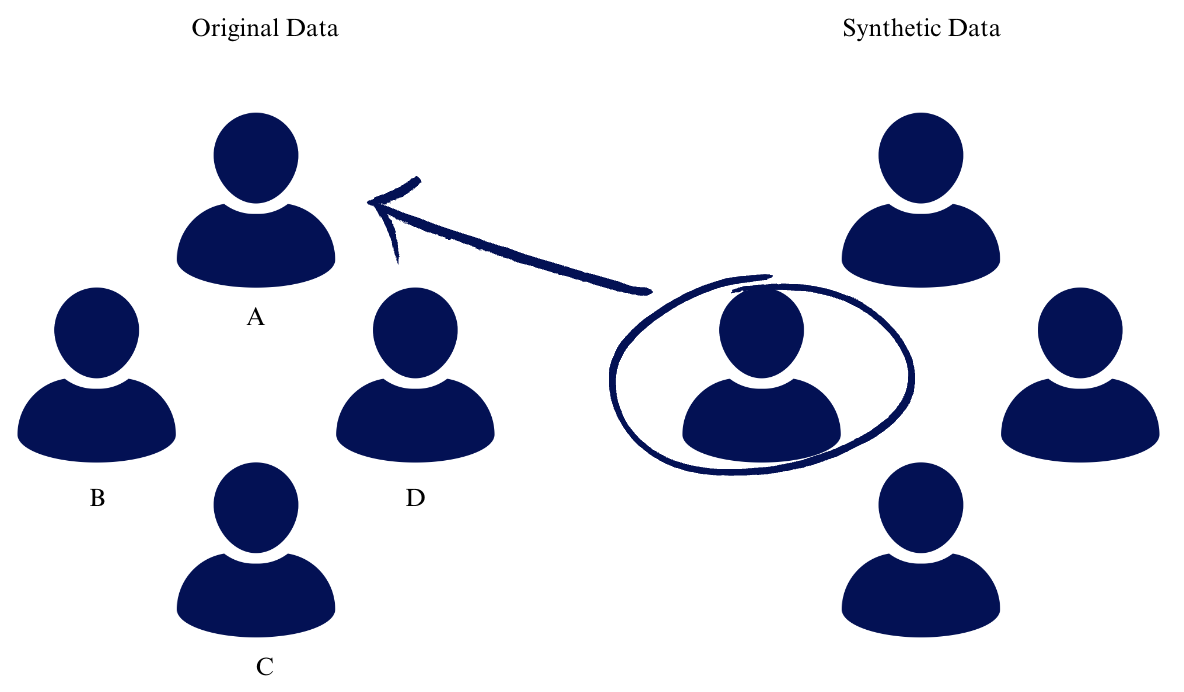
\includegraphics[width=0.5\textwidth]{Images/Reidentificationrisk.png}
    \caption{Re-identification risk}
    \label{fig:synthesis_1}
\end{figure}
\vspace{10pt}

\textbf{Membership inference risk} \\
Membership inference risk refers to the probability that an attacker can determine whether a specific individual's data was included in a dataset used to train a machine learning model or generate synthetic data \cite{hyeong2022empirical}. Such knowledge could reveal sensitive information about individuals, even if the data itself is anonymised. Understanding and mitigating this risk is essential for ensuring privacy in data sharing and open science practices.

\vspace{10pt}
\begin{figure}[H]
    \centering
    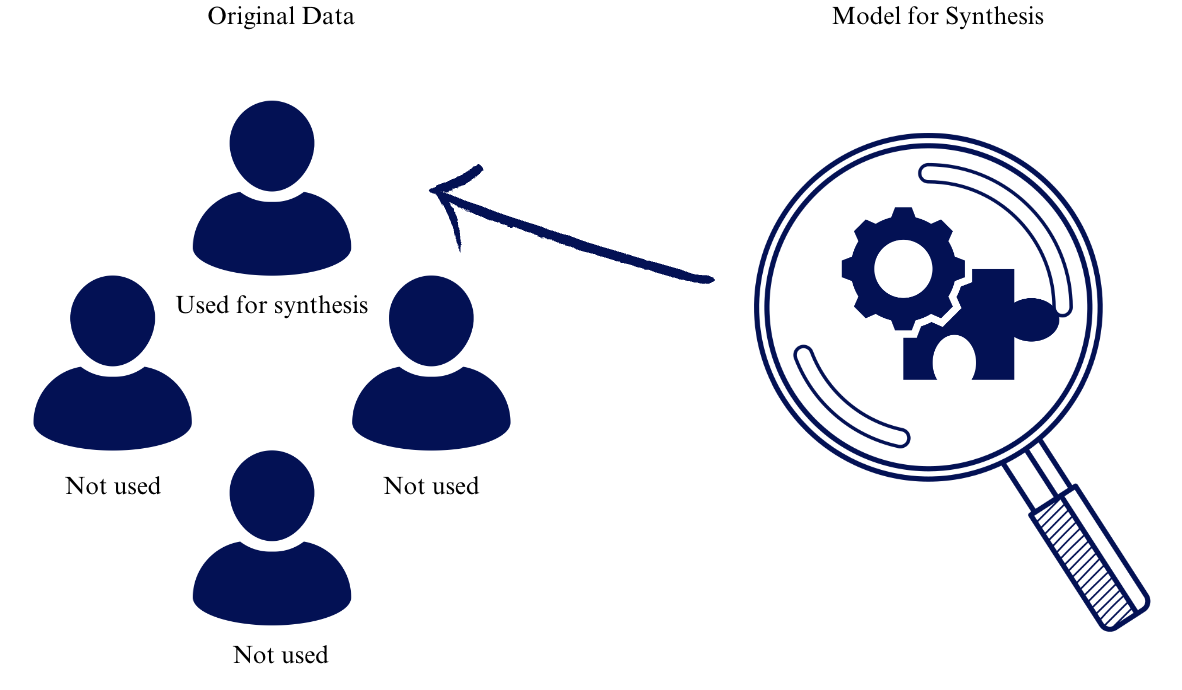
\includegraphics[width=0.5\textwidth]{Images/membershipinference.png}
    \caption{Membership inference risk}
    \label{fig:synthesis_1}
\end{figure}
\vspace{10pt}

\textbf{Attribute disclosure risk}\\
Attribute disclosure risk pertains to the likelihood that sensitive or private information about individuals can be inferred from a dataset, even if direct identifiers are removed. This risk arises when the remaining attributes in the dataset allow an observer to deduce specific details about individuals \cite{hittmeir2020baseline}. For instance, if a dataset includes a combination of age, zip code, and occupation, it might still reveal sensitive information about individuals, such as their income or health status. As such, attribute disclosure risk is similar to the re-identification risk. Yet, whereas the re-identification risk focuses on identifying individuals from data, attribute disclosure risk focuses on revealing sensitive attributes in particular. 

\textbf{Testing for Privacy Risks}\\
For each of these risks, various methods exist on how to measure them. These methods range from manually comparing records from the original dataset with records from the synthetic dataset based on quasi-identifiers, or checking whether outliers in the synthetic dataset can be linked to outliers in the original dataset to statistically measuring risks and mitigating them. Statistical tests can compare the similarities and differences between both the synthetic and original dataset, for example by calculating statistical distance measures. Examples are Euclidean distance, which connects each record in the synthetic dataset with the most similar record of the original dataset \cite{hittmeir2019utility}, or Bayesian estimation methods \cite{hu2018bayesian}. Another common method for measuring these risks is to simulate attacks on the privacy of the synthetic dataset. In these scenarios, models are trained to act as adversaries that aim to gain sensitive information from the synthetic dataset. These models, controlled by the researchers, can help to identify weak points in the synthetic data and quantify potential privacy risks \cite{boudewijn2023privacy,van2023membership,hittmeir2020baseline}.

 \subsection{The issue: lack of standards for privacy}
 Although there are a multitude of methods and techniques to evaluate the privacy of a generated synthetic dataset, there are currently several challenges that need to be addressed. 
 
 \textbf{Individualised data generation processes} \\
 Each generation of synthetic data involves unique processes tailored to specific use cases, datasets, and goals. Consequently, the techniques and methods used for calculating privacy risks can vary widely. This variability means that there is no one-size-fits-all approach for assessing privacy, and each synthetic data generation scenario may require a distinct set of privacy evaluation methods. This individualised approach complicates efforts to compare and validate privacy measures across different studies and applications.
 
 \textbf{Absence of standardised risk thresholds} \\
Possibly due to the complexity and variety of synthetic data generation methods and use cases, there are currently no universally accepted standards for defining what constitutes \textit{high} risk or \textit{low} risk in the context of privacy measures. Different techniques for evaluating privacy, such as re-identification risk or membership inference risk, may use varying thresholds to categorise risk levels. This lack of standardised thresholds creates inconsistencies in privacy assessments, making it challenging to interpret results and apply them consistently across different research contexts. Another hurdle is the difference between quantitative measures of privacy risks compared to the evaluation of privacy officers, lawyers or other experts in the field, who may hold different standards for risk thresholds than statistical measures and whose standards may differ per organisation or individual. Thus, potentially conflicting legal, ethical, statistical and organisational thresholds for privacy may hinder data scientists or researchers to develop synthetic data that can be used and shared. 
 
 \textbf{Evolving nature of synthetic data generation} \\
 The field of synthetic data generation is rapidly advancing, with new methods and techniques continually emerging. As a result, established privacy evaluation methods may become outdated or less effective over time. This constant evolution complicates the development and maintenance of standard practices for privacy assessments, as researchers must continually adapt their approaches to keep pace with technological advancements and emerging privacy risks.

 \subsection{Increasing privacy through differential privacy}
 Differential privacy is a mathematical framework used to provide privacy guarantees when releasing information about a dataset. It ensures that the output of a synthetic dataset does not significantly change when any single individual's data is added or removed, thus protecting individual privacy. In this framework, privacy is measured through two parameters: $\epsilon$ (epsilon) and $\delta$ (delta). $\epsilon$ measures the privacy loss, whereas $\delta$ represents the probability of the privacy guarantee being violated. In practice, differential privacy can be applied by determining the desired levels of privacy based on the sensitivity of the data and the acceptable risk and applying the associated values for both $\epsilon$ and $\delta$. Depending on the chosen values for $\epsilon$ and $\delta$, noise is added to the synthetic dataset, meaning that random modifications are made to the data to obscure the contributions of individual data points. While differential privacy is a robust technique for protecting individual privacy in datasets, it has notable drawbacks, in particular in relation to the framework's complexity. Implementing differential privacy requires careful tuning of privacy parameters, which can be complex and context-dependent. This complexity can make it difficult for researchers without extensive expertise in privacy-preserving techniques to apply differential privacy effectively \cite{dwork2006differential}
 

\section{Utility of synthetic data}

Specifically in the context of open science, the utility of synthetic data is paramount, as it must not only preserve privacy but also effectively support research objectives. Utility measures are used to evaluate how well synthetic data replicates the original data's characteristics and supports scientific analysis. These measures ensure that while data privacy is maintained, the synthetic data remains valuable for the intended use cases. What constitutes \textit{valuable} may differ per use case and goal for the synthesis. The following measures are some of the most common utility measures:

\textbf{Statistical accuracy} \\
One of the primary utility measures is statistical accuracy, which assesses how well synthetic data reflects the statistical properties of the original dataset. This is often also called fidelity. Specifically, this means that synthetic datasets should accurately capture the distribution and relationships of key variables. Techniques such as the Kolmogorov-Smirnov test or Chi-Square, or simple visualisations, can be used to test and compare distributions between synthetic and real datasets, ensuring that synthetic data replicates these characteristics accurately. Correlation coefficients, like Pearson's or Spearman's rank correlation, help verify that relationships between variables are preserved. Accurate statistical representation is crucial for ensuring that synthetic data can be used effectively in a wide variety of scientific research where data integrity is vital \cite{dankar2021fake,el2020seven,arnold2020really}.

\textbf{Utility in data analysis and decision-making} \\
Synthetic data should support meaningful analysis and visualisation. For example, replication studies with synthetic data of studies using the original data should generate the same general results \cite{braddon2023exploring}. Researchers can also apply clustering or classification models to synthetic data and compare the results with those obtained from real data. Consistent findings suggest that synthetic data is useful for generating insights and conducting robust scientific analysis. Furthermore, synthetic data should lead to valid and actionable conclusions, reinforcing its utility in practical application. Two problems with using these types of utility measures is that they are inherently use-case dependent and require the original data as a comparison. Thus, when synthetic data created for data analysis is shared and used by others, it may become less useful when not used for similar tasks.

\textbf{User experience and interpretability} \\
Finally, the ease of use and interpretability of synthetic data are essential utility measures. For open science, synthetic data must integrate smoothly into existing research workflows and tools. It should be formatted in a way that is compatible with FAIR standards.


\section{The trade-off between privacy and utility}

Specifically in the context of open science, researchers may generate synthetic data with the goal to create a dataset that both preserves the privacy of the original data, whilst also creating a synthetic dataset that strongly mimics the original data, to enhance utility for statistical analysis, informational purposes or other use cases. However, researchers have to take into account a potential trade-off between utility and privacy.

The core of the trade-off lies in the fact that increasing utility often comes at the cost of decreased privacy protection, and vice versa. Specifically, such a trade-off could appear if the model through which the synthetic data is generated is \textit{overfitting}, thus mimicking the original data so well that - by chance - one or more records in the synthetic dataset have the exact same characteristics as ones in the original data. Conversely, as privacy safeguards become more stringent, for example by adding noise to the synthetic dataset, the synthetic data may become less representative of the original data, leading to potential inaccuracies in research findings. Finding an optimal balance requires careful consideration of both privacy needs and objectives for the synthetic data. The acceptable level of privacy and utility may vary per use case and context. Ultimately, the goal is to achieve a synthesis of data that adequately protects privacy while still providing valuable insights and supporting robust scientific research. This balancing act is essential for advancing open science while ensuring that individual privacy remains protected. 

\begin{figure}[H]
    \centering
    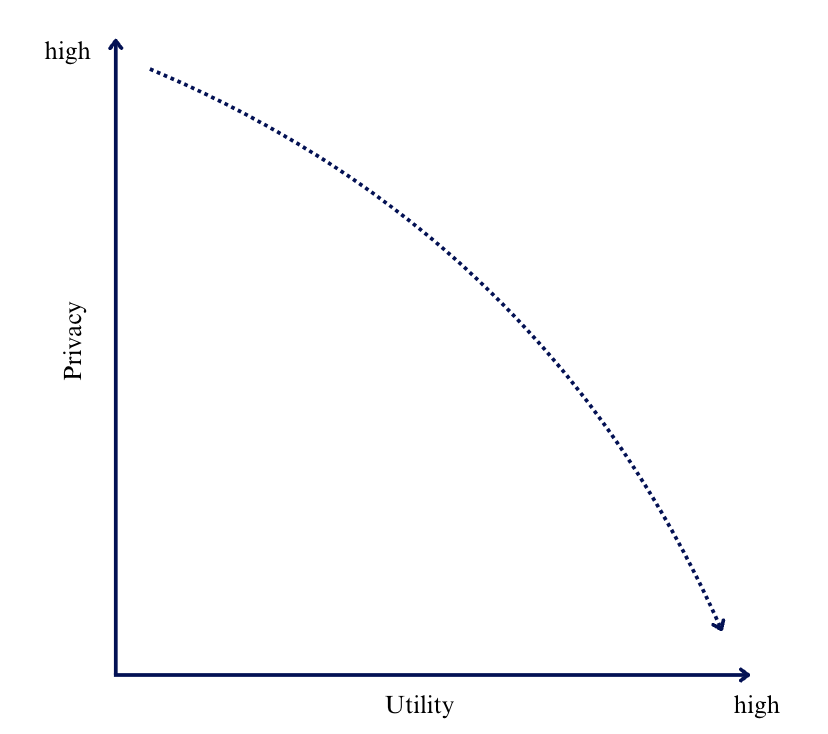
\includegraphics[width=0.8\textwidth]{Images/Screenshot 2024-08-06 at 13.06.13.png}
    \caption{Privacy-utility trade-off.}
    \label{fig:synthesis_1}
\end{figure}














